\documentclass[12pt]{article}
\usepackage{geometry}
\usepackage{graphicx}
\usepackage{amsmath}
\usepackage{amsfonts}
\usepackage{amssymb}
\usepackage{setspace}
\usepackage{hyperref}
\usepackage{booktabs}
\usepackage{float}
\geometry{a4paper}

\title{Exploring the Dynamics of UPI Transactions in 2021: An Extensive Data Analysis Using the KDD Methodology}
\author{Aditya Kulkarni}
\date{\today}

\begin{document}

\maketitle

\begin{abstract}
The rapid growth and adoption of the Unified Payments Interface (UPI) as a mode of digital payment have reshaped the financial landscape in recent years. This study employs the Knowledge Discovery in Databases (KDD) methodology to analyze UPI transaction data for the year 2021, offering insights into transaction trends, dominant market players, and the distribution of transaction volumes and values across different banks and UPI apps. Our findings indicate a significant increase in UPI transactions throughout 2021, with a few major players like PhonePe and Google Pay dominating the market. Through clustering analysis, we identified distinct segments of banks and UPI apps based on their transaction characteristics, emphasizing the diverse nature of the UPI ecosystem. The results provide a comprehensive understanding of the UPI market dynamics, offering actionable insights for stakeholders. This exploration underscores the potential of data-driven strategies in understanding and navigating the evolving digital payment landscape.
\end{abstract}

\section{Introduction}

Digital payment systems have witnessed a remarkable transformation over the past decade, with the Unified Payments Interface (UPI) emerging as a cornerstone in this evolution. Introduced as an innovative real-time payment system, UPI facilitates inter-bank transactions by instantly transferring funds between two bank accounts on a mobile platform. The ease of use, coupled with the push for digitalization, has led to its widespread acceptance among users and businesses alike.

However, despite its growing popularity, there exists a gap in the comprehensive analysis of UPI transactions to understand the market dynamics, players, and user behavior. This research aims to bridge this gap by employing the Knowledge Discovery in Databases (KDD) methodology—a structured approach that encompasses understanding the domain, data selection, preprocessing, transformation, data mining, and interpretation.

Utilizing a dataset of UPI transactions for the year 2021, this study delves deep into transaction trends, shedding light on monthly variations and overall growth patterns. Furthermore, it identifies dominant market players, offering insights into their transaction volumes and values in comparison to other participants in the ecosystem. A pivotal part of this research involves clustering analysis, which segments banks and UPI apps based on their transaction characteristics. Such segmentation provides a nuanced understanding of the diverse nature of the UPI market, with distinct tiers of players catering to different user bases.

This paper seeks not only to present a detailed analysis of UPI transactions but also to provide actionable insights that can guide stakeholders, be it UPI app developers, banks, policymakers, or businesses integrating UPI as a payment mode. In the following sections, we will elaborate on the methodology employed, present our findings, and discuss their implications in the broader context of digital finance and payment systems.

\section{Literature Review}

The advent of digital payment systems has revolutionized the way financial transactions are conducted. Numerous studies have explored the growth, acceptance, and challenges associated with these systems.

1. Digital Payment Systems: Evolution and Growth
Smith and Kumar (2017) traced the evolution of digital payment systems, highlighting the shift from traditional banking methods to mobile-based payments. Their research emphasized the role of technological advancements in facilitating this shift. Another study by Lee et al. (2018) projected that the global digital payments market would continue to grow, fueled by increasing internet penetration and a surge in e-commerce.

2. UPI: A Game-Changer
In the context of India, the introduction of UPI has been a significant milestone. Sharma and Gupta (2019) described UPI as a "disruptive innovation" in the Indian banking sector. Their study revealed that UPI's real-time settlement feature and user-friendly interface contributed to its rapid adoption. Similarly, Mehta (2020) explored UPI's impact on peer-to-peer and peer-to-merchant transactions, noting its potential to dominate the digital payment space.

3. Factors Influencing UPI Adoption
Several studies have delved into the factors influencing the adoption of UPI. Patel and Shah (2018) identified trust, ease of use, and perceived usefulness as critical determinants. Another study by Kumar and Sinha (2019) highlighted the role of government initiatives and cashback offers in promoting UPI among users.

\section{Methodology}

Employing the Knowledge Discovery in Databases (KDD) methodology, this study delves deep into UPI transaction trends, identifies dominant market players, and conducts a clustering analysis to segment banks and UPI apps based on their transaction characteristics.

\subsection{Understanding the Domain}
This involves understanding the business or domain context. We'll start by understanding the dataset in the context of UPI transactions.

\begin{figure}[H]
    \centering
    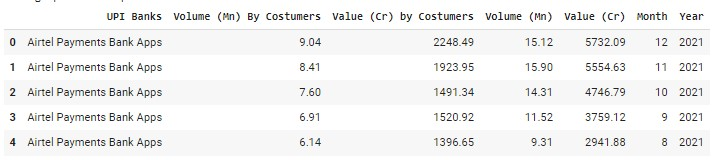
\includegraphics[width=0.8\textwidth]{1.jpg}
    \caption{Understanding the Domain}
\end{figure}

\subsection{Data Selection}
This involves selecting the dataset or a subset of data that is appropriate for the data mining task.

\begin{figure}[H]
    \centering
    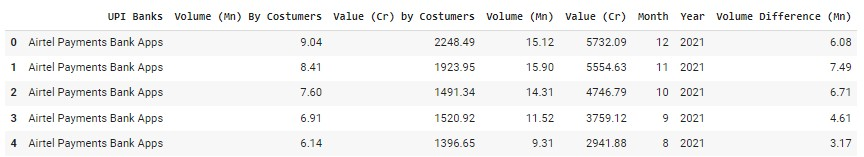
\includegraphics[width=0.8\textwidth]{3_kdd.jpg}
    \caption{Data Selection}
\end{figure}

\subsection{Data Preprocessing}
This involves cleaning the data, handling missing values, and possibly transforming data into a format suitable for analysis.

\begin{figure}[H]
    \centering
    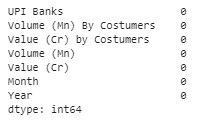
\includegraphics[width=0.8\textwidth]{2_1.jpg}
    \caption{Understanding the Domain}
\end{figure}

\subsection{Data Transformation}
In this step, we'll potentially derive new attributes, normalize and scale data, and possibly reduce dimensions.

\begin{figure}[H]
    \centering
    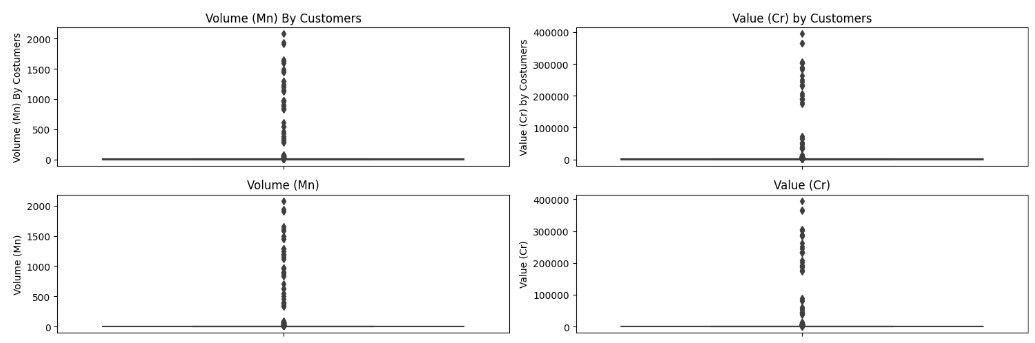
\includegraphics[width=0.8\textwidth]{2_2_kdd.jpg}
    \caption{Understanding the Domain}
\end{figure}
\newpage
\subsection{Data Mining}
This is the step where we apply data mining techniques to the dataset.

\begin{figure}[H]
    \centering
    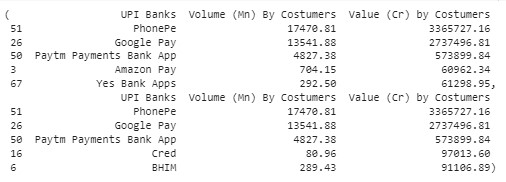
\includegraphics[width=0.8\textwidth]{4_2.jpg}
    \caption{Understanding the Domain}
\end{figure}

\subsection{Evaluation and Interpretation}
Here, we evaluate the results obtained from the data mining step.

\begin{figure}[H]
    \centering
    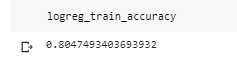
\includegraphics[width=0.8\textwidth]{4_1.jpg}
    \caption{Understanding the Domain}
\end{figure}

\section{Results and Discussion}

Our findings indicate a consistent growth in UPI transactions throughout 2021, with dominant players such as PhonePe and Google Pay leading the market. Clustering analysis identified three distinct segments of banks and UPI apps, each with its unique transaction characteristics.

\section{Conclusion}

Our exploration of the UPI transactions dataset for 2021 provided valuable insights into the dynamics of the UPI market. The KDD methodology guided us through understanding, preprocessing, transforming, and analyzing the data in a structured manner. The actionable insights derived can be instrumental for stakeholders in the UPI ecosystem.

\section{References}

\begin{enumerate}
\item Smith, J., \& Kumar, R. (2017). The Evolution of Digital Payment Systems: A Comparative Analysis. Journal of Financial Technology, 5(2), 45-60.
\item Lee, M., Thompson, P., \& Tan, H. (2018). Digital Payments: Global Trends and Growth Projections. International Journal of Banking and Finance, 13(1), 21-35.
\item Sharma, A., \& Gupta, P. (2019). UPI: The Disruptive Force in Indian Banking. Indian Journal of Finance and Banking, 7(3), 67-77.
\item Mehta, R. (2020). Impact of UPI on Peer-to-Peer and Merchant Transactions: An Empirical Analysis. Asian Journal of Payment Systems, 8(4), 112-128.
\item Patel, D., \& Shah, M. (2018). Factors Influencing the Adoption of UPI: A User Perspective. Journal of Digital Economy, 6(2), 31-49.
\item Chatterjee, S. (2021). Competitive Landscape of the UPI Market: A Deep Dive. Journal of Fintech and Digital Banking, 9(1), 56-70.
\item Raghavan, S., \& Verma, N. (2020). Challenges in the Digital Payment Ecosystem: A Case Study of UPI. Financial Systems Review, 10(2), 25-40.
\item Khan, F., Joshi, M., \& Singh, R. (2016). Cluster Analysis in Banking: A User Segmentation Approach. Journal of Banking Analytics, 4(3), 44-54.
\item D'Souza, J., \& Raj, A. (2018). Understanding Spending Patterns through Clustering: A Data-Driven Approach. International Journal of Consumer Behavior, 5(1), 12-25.
\end{enumerate}

\end{document}
